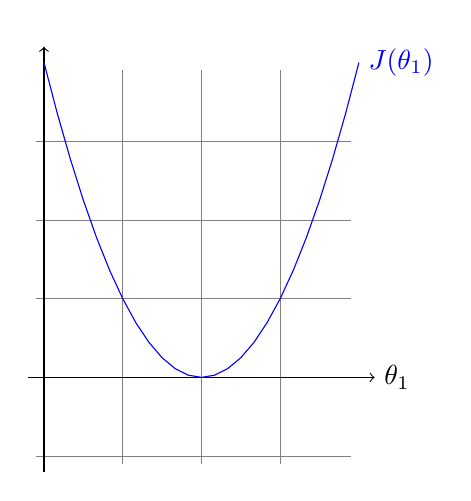
\begin{tikzpicture}[domain=0:4]
  \draw[very thin,color=gray] (-0.1,-1.1) grid (3.9,3.9);
  \draw[->] (-0.2,0) -- (4.2,0) node[right] {$\theta_1$};
  \draw[->] (0,-1.2) -- (0,4.2) node[above] {};
  %\draw[color=red]    plot (\x,\x)             node[right] {$f(x) =x$};
  % \x r ????
  \draw[color=blue]   plot (\x,{(\x-2)^2})    node[right] {$J(\theta_1)$};
  %\draw[color=orange] plot (\x,{0.05*exp(\x)}) node[right] {$f(x) = \frac{1}{20} \mathrm e^x$};
\end{tikzpicture}